\section{Empirical analysis of improvement}

In order to empirically assess the space efficiency of our improvement, we
measured the size of the interlink data structure in the case of interlink
\emph{lists}, the previously proposed format, and in the case of interlink
\emph{sets}, our newly proposed format. Our results are illustrated in
Figure~\ref{fig.set-list-vector-comparison}.

Based on the theoretical analysis of Section~\ref{sec.construction}, we expected
to see approximately an improvement of $50\%$ in this structure.

\begin{figure}
   \centering
   \subcaptionbox[]{%
      \centering
      Bitcoin
   }
   [
       0.80\textwidth
   ]
   {
       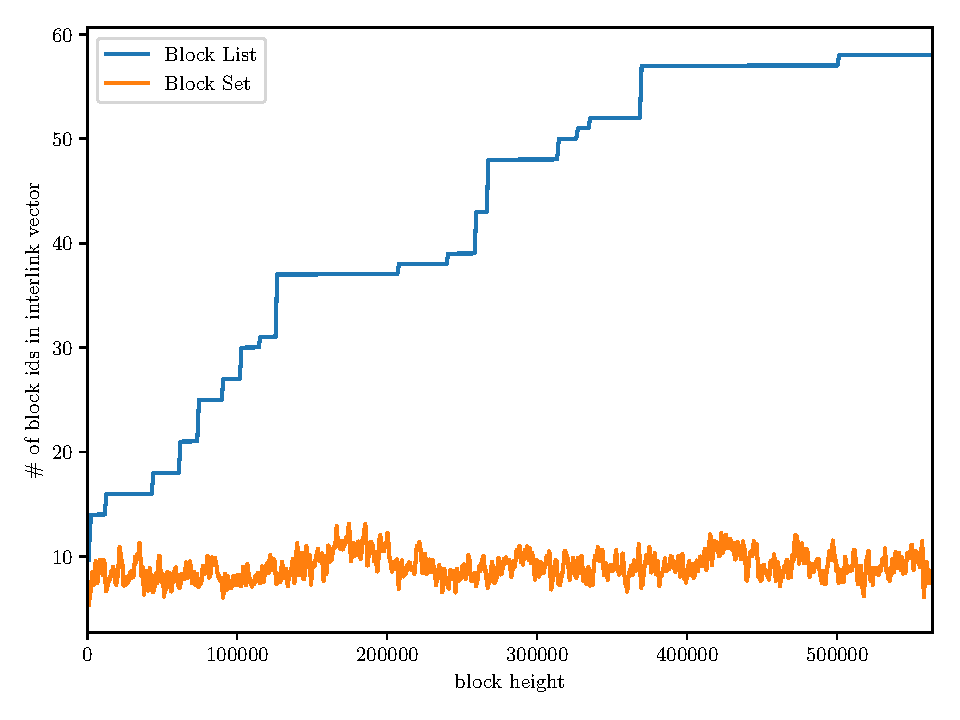
\includegraphics[width=0.85 \textwidth]
       {figures/interlink-vector-blocklist-vs-blockset.pdf}
   }
   \vskip 0pt
   \subcaptionbox[]{%
      \centering
      Litecoin
   }
   [
       0.80\textwidth
   ]
   {
       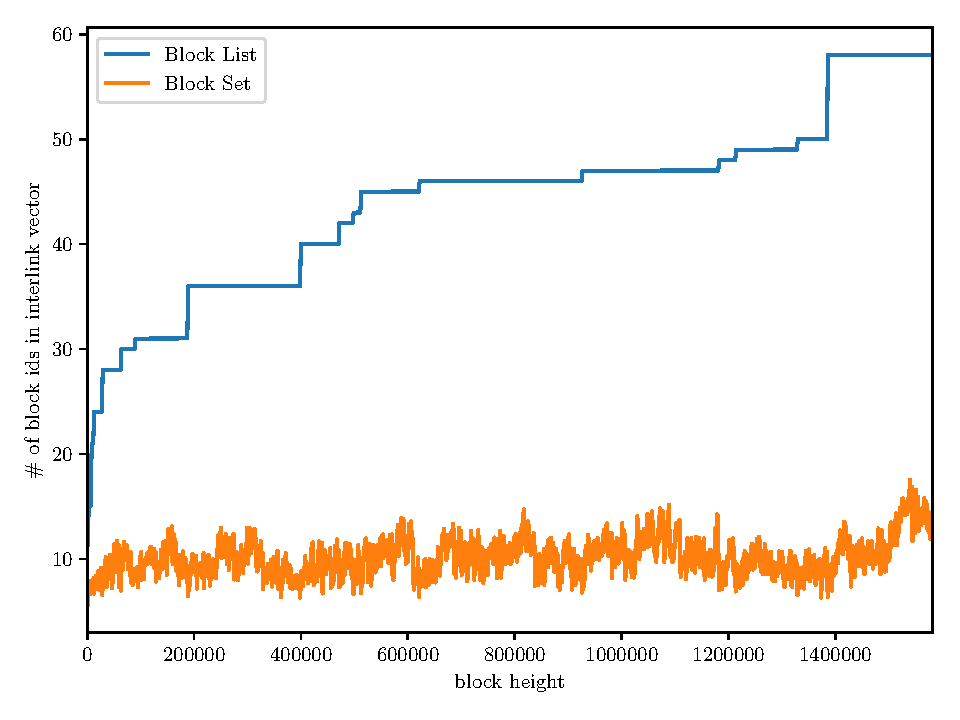
\includegraphics[width=0.85 \textwidth]
       {figures/interlink-vector-blocklist-vs-blockset-litecoin.pdf}
   }
   \caption{A comparison of interlink vector sizes for interlink block lists (previous work) and interlink block sets (this work) in two popular blockchains (lower is better)}
   \label{fig.set-list-vector-comparison}
\end{figure}

\begin{figure*}[h]
\begin{center}
  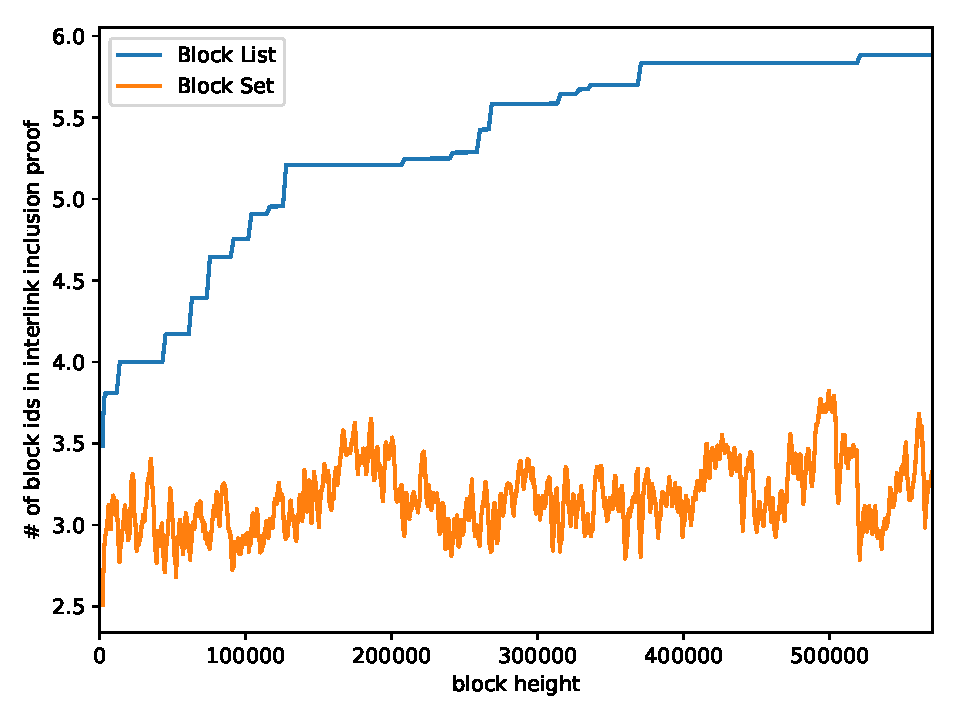
\includegraphics[width=0.95\textwidth]{figures/interlink-proof-list-vs-set.pdf}
  \caption{A comparison of a proof-of-inclusion size in the case of interlink block lists (previous work) and interlink block sets (this work) in Bitcoin (lower is better)}
  \label{fig.set-list-proof-comparison}
  \end{center}
\end{figure*}

\TODO{TODO: Explain gains attained due to variable difficulty}
